\documentclass[twopage,12pt,a4paper]{report}
\linespread{1.5}
\usepackage[toc,page]{appendix}
\usepackage[T1]{fontenc}
\usepackage[utf8]{inputenc}
\usepackage{mathptmx}
\usepackage{amsmath}
\usepackage{amsfonts}
\usepackage{amssymb}
\usepackage{makeidx}
\usepackage{graphicx}
\usepackage{multirow}
\usepackage{epstopdf}
\usepackage{setspace}
\usepackage{listings}
\usepackage{chemformula}
\usepackage{graphicx}
\usepackage[document]{ragged2e}
\usepackage{color} %red, green, blue, yellow, cyan, magenta, black, white
\definecolor{mygreen}{RGB}{28,172,0} % color values Red, Green, Blue
\definecolor{mylilas}{RGB}{170,55,241}
%\usepackage[a4paper, vmargin={5cm,3cm}, hmargin={3cm,2cm}]{geometry}
\usepackage{subfigure}
\usepackage{longtable}
%\usepackage{natbib}
\usepackage{caption}
\newcommand\nomenclature[2]{#1 & #2 \\}
%-------------------
\usepackage{tikz}
\usetikzlibrary{arrows,shapes}
\usetikzlibrary{fadings}
\usepackage{textpos}
\usepackage{graphicx}
\usepackage{mathtools}
\usepackage{amsmath}
\usepackage{arydshln}   %%% package for dotted line
\usepackage{algorithmic}
%--------------------

\usepackage{vmargin}
\setpapersize{A4}
\setmarginsrb{25mm}{20mm}{2mm}{22mm}{3mm}{12mm}{3mm}{10mm}

\setlength{\parsep}{10pt}
\setlength{\textwidth}{160mm}
\setlength{\textheight}{245mm}
%\usepackage[Lenny]{fncychap}
%\usepackage[Bjornstrup]{fncychap}
\usepackage[breaklinks]{hyperref}
\hypersetup{
    colorlinks,%
    citecolor=black,%
    filecolor=black,%
    linkcolor=black,%
    urlcolor=black
}


\begin{document}
\begin{raggedright}
\justify
\thispagestyle{empty}
\begin{center}

\huge
\textbf{ Implementation of LDPC decoder using AHIR tool chain  }\\
\bigskip
\bigskip
\bigskip

\normalsize

\vspace*{3cm}

\begin{Large}
Submitted By\\
\end{Large}

\begin{LARGE}
\textbf{Anurag Gupta\\(Roll No. 153070050)}\\
\end{LARGE}
\begin{Large}
Under the Guidance of\\ 
\end{Large}
\vspace*{4mm}
\begin{LARGE}
\textbf{Prof. Madhav P. Desai}
\end{LARGE}
\bigskip

\begin{figure}[h!]
 \centering
 
\includegraphics[width=7cm]{iitb}

\end{figure}



\large
\textbf{Department of Electrical Engineering}\\
\bigskip
\textbf{INDIAN INSTITUTE OF TECHNOLOGY BOMBAY}\\
\bigskip
\textbf{2017}
\end{center}

\normalsize



 \pagenumbering{roman}  % 1, 2, 3, 4, ...
\setcounter{page}{1}
\tableofcontents
\cleardoublepage 

\clearpage


\begin{abstract}
   We describe a complete procedure of testing The Kintex®-7 family FPGA KC705. Xilinx provides documentation for testing the kit for Windows operating system. We need to test the Xilinx card using Ubuntu OS. The document presents step by step procedure for setting up a workstation with Ubuntu OS and then testing KC705 FPGA card.
   First we explained prerequisites for testing FPGA card. The Prerequisites explains how to install Ubuntu ,Cable Drivers and ISE .
   Then we performed three tests set-ups to check the functionality of FPGA card. 
   The first test set-up is Built-in-self-test. BIST comprise of twelve tests. Those tests are UART test,LED test, IIC test, FLASH test, TIMER test,ROTARY test,SWITCH test,LCD test,DDR3 External Memory test,BRAM Internal Memory test,ETHERNET loopback test,BUTTON test. 
   The second test set-up is for Ethernet test and third test set-up is for PCIe test, through which we test throughput by Ethernet link and PCIe link respectively. 
   
\end{abstract}



% chapter 1
%%%%%%%%%%%%%%%%%%%%%%%%%%%%%%%%%%%%%%%
\chapter{Introduction}
\pagenumbering{arabic}  % 1, 2, 3, 4, ...
\setcounter{page}{1}
%----------------------------------------------

The Low Density Parity Check (LDPC) codes are error correcting codes used in communication systems. 
These codes were first proposed by Gallager in 1962.\textbf{[]} 
Due to computational limitations potential of these codes were not exploited at that time. Meanwhile block codes and convolution codes were used for error correction, but their performance fell short from the theoretical limit set by Shannon.\textbf{[] }
In year 1992 researcher Mckey and Neal discovered new class of block codes that outperformed the  state of art turbo codes. 
Soon it was recognized that is these codes are rediscovery of LDPC codes proposed by Gallager. Many researchers
including Luby, Mitzenmacher, Shokrollahi, Spielman, Richardson and Urbanke, produced new irregular LDPC codes\textbf{[]} and these codes become popular due to there rate approaching to channel capacity.
The best codes approaching to Shannon limit was discovered by Sae-Young Chung, for a white Gaussian noise channel threshold obtained was within 0.0045 dB of
the Shannon limit with block length of $10^7$ at a bit error rate of $10^-6$. \textbf{[] }
Nowadays LDPC codes are used in DVB-S2 standard for the satellite transmission of digital television. \textbf{[]} LDPC codes are also used for 10GBase-T Ethernet, a part of the Wi-Fi 802.11 standard as an optional part of 802.11n and 802.11ac, in the High Throughput (HT) PHY specification.\textbf{[]}

\chapter{Theory of LDPC}


The goal of communication is to transmit a message and receive it correctly even after noisy transmission through the channel. This is achieved by introducing redundancy in the message at the transmitter side, called as encoding of message. The encoded message is called codeword. Then codeword is then transmitted through the noisy channel, which alters the codeword. By some error correcting algorithm the message is extracted back at receiver side, called decoding of the codeword. Thus, the error free transmission takes place by applying error correcting codes in communication system.\\
We have a k bit long message to encode it we introduce a m bit redundancy (or called parity bits) to form a $n(=m+k)$ bit long codeword. These category of codes are called (n,k) block codes. 

\subsection{Parity Check Matrix}

The codeword must satisfy a group conditions to ensure error free transmission or to indicate the error have been taken place. If error occurs, the error can be corrected by applying some algorithm on those group of conditions . The group of conditions are called parity check equations.The matrix form of the condition is called parity check matrix. \\
Example: If a code block $y=[c_1 c_2 c_3 c_4 c_5 c_6]$ has to satisfy following parity check equations. 
\begin{align}
c_1 \oplus c_2 \oplus c_4 =0 \\
 c_2 \oplus c_3 \oplus c_5 =0 \\
c_1 \oplus c_2 \oplus c_3 \oplus c_6 =0 
\end{align}  
Then it's parity check matrix is as follows:
\begin{align}
 H= \left[ \begin{array}{cccccc}
1 & 1 & 0 & 1 & 0 & 0\\
0 & 1 & 1 & 0 & 1 & 0\\
1 & 0 & 0 & 0 & 1 & 1\\
0 & 0 & 1 & 1 & 0 & 1  
\end{array} \right]  
\end{align} 
s.t. $Hy^T=0$.

\subsection{Encoding of Message}
We can rewrite the above equations (1),(2),(3) as:
\begin{align}
c_4 = c_1 \oplus c_2 \\
c_5 = c_2 \oplus c_3 \\
c_6 = c_1 \oplus c_2 \oplus c_3  
\end{align}  
We can find parity check bits $c_4,c_5,c_6$ by message bits $c_1,c_2,c_3$.
Thus we can encode message bits to find codeword. \\
Encoding is preferably done in matrix form, by manipulating parity check matrix to find a generator matrix.
If parity check matrix can be written in the form
$H = [A, I_{n- k} ]$,
where A is an $(n-k)$xk binary matrix and $I_{n-k}$ is the identity matrix of order
$(n-k)$. The generator matrix is then
$G = [I_k , A^T ]$.
s.t $GH^T = 0$. \\
\begin{align}
[c_1 c_2 ... c_6]=[c_1 c_2 c_3] \left[ \begin{array}{cccccc}
1 & 0 & 0 & 1 & 0 & 1\\
0 & 1 & 0 & 1 & 1 & 1\\
0 & 0 & 1 & 0 & 1 & 1  
\end{array} \right]
\end{align}
 

Thus, m is message block containing message bits $[c_1 c_2 c_3]$, then codeword can be generated as $y=mG$.

\subsection{Error Detection \& Correction}

If the codeword got corrupted in the transmission then all the parity check equation will not get satisfied. This we will get $Hy^T\neq0$. The non-zero vector is called syndrome. That shows that received message is corrupted. But there is a certain limit in number of bits upto that error can be detected and corrected.
The limit is represented in term of hamming distance. Hamming distance between two codes is number of flipped bits between them. If $d_{min}$ is minimum distance between codes then maximum number bit flipped to which error can be correctly detected is $d_{min}-1$ and maximum number of bits upto which error can be corrected is
(t) = $[\frac{d_{min}-1}{2}]$
where [] denotes greatest integer function.\\
The more the number of redundant bits the more the hamming distance thus more error bits can be detected and corrected but the code rate is reduces. The correction is directly taking the received vector and comparing it to all the codewords and correcting it to the codeword having minimum distance to it. This is called maximum likelihood decoding. But if n is lager then this task become complex. LDPC maximum likelihood decoding, bit flipping decoding are other decoding schemes which reduce complexity of this task.


\chapter{Generation of different LDPC matrices}

The Bit Error Rate of decoded code word depends upon properties of parity check matrix. A good parity check matrix should be sparse and  it should have good girth.  

Basic parameters to decide of the formation of parity check matrix are as follows . 
\begin{itemize}
\item  \textbf{Random parity check matrix vs systematic parity check matrix:} Parity check matrix that has a specific method of filling $1's$ in matrix are called systematic parity check matrix, else if the position of $1's$ are random, the matrix is called random parity check matrix.
\item\textbf{Regular parity check matrix vs irregular parity check matrix:} Regular parity check matrix has constant number of $1's$ in row and columns, whereas irregular parity check matrix has variable number of $1's$ i its rows and columns. \\
	If $w_c$ is number of $1's$ in a column and $w_r $is number of $1's$ in a row then in a mxn regular parity check matrix
\begin{center}
$ m * ( w_r ) = n * ( w_c ) $ 
\end{center}
%Collectively the set
%v and h is called the degree distribution of the code. 
%\item columns are divided in $w_r$ sets n/$w_r$ columns in each set. 
If we take the fraction of columns
of weight i by $v_i$ and the fraction of rows of weight i by $h_i$ then in a irregular parity check matrix
\begin{center}
$ m * \sum_{i} h_i*i = n *\sum_{i} v_i*i $
\end{center}


\end{itemize} 
%\renewcommand{\labelitemi}{$\square$}
\begin{enumerate}
\item \textbf{Gallager Parity Check Matrix:} \\
Gallager proposed parity check matrix is regular in nature. A regular matrix has constant number of non-zero entries in a row and a column. 
These are represented as (n,$w_c$,$w_r$) codes. where,
\\
$w_c$ = Number of 1\textsuperscript{'}s in a column 
\\
$w_r$ = Number of 1\textsuperscript{'}s in a row 
\\
n = Block length. \\
\textbf{Method of construction:}

o Divide rows in $w_c$ sets with ( m / $w_c$ ) rows in each set.  \\
%\item columns are divided in $w_r$ sets n/$w_r$ columns in each set. 
o All rows of first set of rows contain $w_r$ consecutive once ordered from left to right. \\
o Every other set of row is random column permutation of first set of rows. \\
\textbf{Example of Gallager Matrix:} \\
( n , $w_c$ , $w_r$ ) = ( 12 , 3 , 4 ) ; m = 9 
\[
 H=
 \left[ \begin{array}{cccccccccccc}
1 &  1 &  1  & 1 &  0 & 0 & 0 & 0 & 0 & 0 & 0 & 0 \\
0 & 0 & 0 & 0 & 1 &  1 &  1  & 1 & 0 & 0 & 0 & 0 \\
0 & 0 & 0 & 0 & 0 & 0 & 0 & 0 & 1 &  1 &  1  & 1 \\
-& - & - & - & - & - & - & - & - &  - &  -  & -\\ 
1 &  0 &  1  & 0 &  0 & 1 & 0 & 0 & 0 & 1 & 0 & 0 \\
0 & 1 & 0 & 0 & 0 &  0 &  1  & 1 & 0 & 0 & 0 & 1 \\
0 & 0 & 0 & 1 & 1 & 0 & 0 & 0 & 1 &  0 &  1  &  0\\
-& - & - & - & - & - & - & - & - &  - &  -  & -\\ 
1 & 0 & 0 & 1 & 0 & 0 & 1 & 0 & 0 & 1 & 0 & 0 \\
0 & 1 & 0 & 0 & 0 & 1 & 0 & 1 & 0 & 0 & 1 & 0 \\
0 & 0 & 1 & 0 & 1 & 0 & 0 & 0 & 1 & 0 & 0 & 1 \\ \end{array} \right]  
\]

\item \textbf{Repeat Accumulation Matrix: }

These codes are systematic and irregular. 
Approch of construction is such that each parity-bit can be computed  one  at  a  time  using  only  the  message  bits  and  the  one  previously calculated parity-bit. \\
\textbf{Method of construction:}

o The first (n-m) columns of H correspond to the message bits. Dependency of parity check in over a message bit chosen at random. \\ 
o Rest m columns have  1\textsuperscript{'}s of weight two, that are placed in a step pattern, except the last column which has single 1 as the last entry of the column. \\
%\item columns are divided in $w_r$ sets n/$w_r$ columns in each set. 


 
\textbf{Example of Repeat Accumulation Parity Check Matrix:} \\
  \[ H=
 \left[ \begin{array}{ccccccccccccc}
1 & 0 & 0 &| & 1 & 0 & 0 & 0 & 0 & 0 & 0 & 0 & 0 \\
1 & 0 & 0 &|& 1 & 1 & 0 & 0 & 0 & 0 & 0 & 0 & 0 \\
0 & 1 & 0 &|& 0 & 1 & 1 & 0 & 0 & 0 & 0 & 0 & 0 \\
0 & 0 & 1 &|& 0 & 0 & 1 & 1 & 0 & 0 & 0 & 0 & 0 \\
0 & 0 & 1 &|& 0 & 0 & 0 & 1 & 1 & 0 & 0 & 0 & 0 \\
0 & 1 & 0 &|& 0 & 0 & 0 & 0 & 1 & 1 & 0 & 0 & 0\\
1 & 0 & 0 &|& 0 & 0 & 0 & 0 & 0 & 1 & 1 & 0 & 0 \\
0 & 1 & 0 &|& 0 & 0 & 0 & 0 & 0 & 0 & 1 & 1 & 0 \\
0 & 0 & 1 &|& 0 & 0 & 0 & 0 & 0 & 0 & 0 & 1 & 1 \\ \end{array} \right]  
\] 
Here we can see that $c_4 = c_1$ ;\ $c_5 = c_1 \oplus c_4$ ;\ $c_6 = c_5 \oplus c_2$ ; ...and so on. Thus a parity check depends on a message bit and a previous check bit.
%%%%%%%%%%%%%%%% agorithm template begin %%%%%%%%%%%%%% 



\item \textbf{Quasi-Cyclic (QC) parity Check Matrix: }\\
QC matrix can be construction by 
Sridhara Fuja Tanner (SFT) Method is discussed.\textbf{[]} Performance of quasi-cyclic codes is better for smaller block length, comparable for moderate block length with respect to random-regular codes.\\
Method of Construction of (j,k)-regular QC-LDPC code:
\begin{itemize}
\item Construct two sequences $\{s_1,s_2,...,s_{j-1}\}$ and $\{t_1,t_2,...,t_{k-1}\}$, whose elements are randomly selected from GF(p), where p is prime and p$>$2 , $s_i \neq s_x \ \& \ t_i \neq t_x$ if i $\neq$x.
\item Now, form a preliminary matrix Y with the elements of GF(p) as follows:
\begin{align}
 E= \left[ \begin{array}{cccc}
e_{0,0} & e_{0,1} & \cdots & e_{0,k-1} \\
e_{1,0} & e_{0,1} & \cdots & e_{0,k-1} \\
\vdots & \vdots & \ddots & \vdots \\
e_{j-1,0} & e_{j-1,1} & \cdots & e_{j-1,k-1} 
\end{array} \right] 
\end{align}
 
where (i,j)th element of E is calculated by following quadratic congruential equation for a fix parameter
$\kappa\epsilon\{1,2,...,p-1\} $ and $\nu_i,\nu_j\epsilon\{1,2,...,p-1\} $: 
\begin{align}
 e_{i,j}=[\kappa(s_i+t_j)^2 + \nu_i +\nu_j] 
\end{align}
\item So the parity check matrix H is represented by jxk array of circulant permutation of identity matrix. 
\[
 H= \left[ \begin{array}{cccc}
I(e_{0,0}) & I(e_{0,1}) & \cdots & I(e_{0,k-1}) \\
I(e_{1,0}) & I(e_{0,1}) & \cdots & I(e_{0,k-1}) \\
\vdots & \vdots & \ddots & \vdots \\
I(e_{j-1,0}) & I(e_{j-1,1}) & \cdots & I(e_{j-1,k-1}) 
\end{array} \right] \]

 
Where I(x) is pxp identity matrix with row cyclically shifted right by x position.
\end{itemize}


\item \textbf{Mckey Neal Parity Check Matrix: }\\
Mckey Neal proposed regular (n,$w_c$,$w_r$) construction of codes using random distribution of non-zero entries. These codes have better performance for large block length compared to other codes.
Method of construction:
\begin{itemize} 
\item Start from the first column.Place $w_c$ 1\textsuperscript{'}s in the column randomly and track number of 1\textsuperscript{'}s in a row.
\item Repeat the process for other columns. Break only if at any point number of 1\textsuperscript{'}s in the row becomes greater than $w_r$.
\item If break occurs then go back to some columns and repeat algorithm till all columns get filled.
\end{itemize} 
\textbf{Example:}\\
 n = 12, m = 9  
  \[H=
 \left[ \begin{array}{cccccccccccc}
1 & 0 & 0 & 0 & 0 & 1 & 0 & 1 & 0 & 1 & 0 & 0 \\
1 & 0 & 0 & 1 & 1 & 0 & 0 & 0 & 0 & 0 & 1 & 0 \\
0 & 1 & 0 & 0 & 1 & 0 & 1 & 0 & 1 & 0 & 0 & 0 \\
0 & 0 & 1 & 0 & 0 & 1 & 0 & 0 & 0 & 0 & 1 & 1 \\
0 & 0 & 1 & 0 & 0 & 0 & 1 & 1 & 0 & 0 & 0 & 1 \\
0 & 1 & 0 & 0 & 1 & 0 & 0 & 0 & 1 & 0 & 1 & 0\\
1 & 0 & 0 & 1 & 0 & 0 & 1 & 0 & 0 & 1 & 0 & 0 \\
0 & 1 & 0 & 0 & 0 & 1 & 0 & 1 & 0 & 1 & 0 & 0 \\
0 & 0 & 1 & 1 & 0 & 0 & 0 & 0 & 1 & 0 & 0 & 1 \\ \end{array} \right]  
\] 

Mackay Neal construction can be adapted to avoid cycles of length 4, called 4-cycles.\\
Method to avoid 4-cycles:
\begin{itemize}
\item Generate a preliminary parity check matrix.
\item Add 1s to check matrix in the rows that have no 1s in them, hence are redundant, or that have only one 1 , in which case corresponding codeword bits will always be zero. The places in these rows to add 1s are selected randomly. 
\item Choose odd number of 1s to put in a column. If preliminary parity check matrix constructed has an even number of 1s in each column, problem may occur that will cause the rows to add to zero, and hence at least one check will become redundant.
\item To eliminate situation where a pair of columns both have 1s in a particular pair of rows, which correspond to cycles of length four in the factor graph, one of the 1s involved is moved randomly within its column.
\end{itemize}
Avoiding the cycles increase the girth of the graph thus helps to converge the iterative decoding faster.  
%%%%%%%%%%%%%%%%%%%%%%%%%%%%%%%%%%%%%%%%%%%%%%%%%%
\end{enumerate} %end of parity check matrix type
\chapter{Decoding Algorithms}
\subsection{Message Passing Decoding}
The algorithms used to decode LDPC codes are iterative in nature. In every iteration some information has to be passed through the edge of the bipartite graph(Tanner graph), representing corresponding parity check matrix. Thus these type of iterative algorithm are generally termed as message passing decoding.\\
Two type of message passing decoding algorithms are discussed. Bit flipping algorithm takes hard decision at the received information and then principally uses majority whereas belief propagation algorithm uses soft information or the probabilistic approach.\\
LDPC codes are often represented in graphical form by a Tanner graph.
The Tanner graph consists of two sets of vertices.
n vertices for the codeword
bits (called bit nodes), and m vertices for the parity-check equations (called
check nodes).
An edge joins a bit node to a check node if that bit is included
in the corresponding parity-check equation. Number of edges in the
Tanner graph is equal to the number of ones in the parity-check matrix. Notion of Tanner graph was given by Tanner \textbf{[]} \\
Example:


\[
 H =  \left[ \begin{array} {c|cccccccc} 
  &    B1 &   B2 &   B3 &  B4  &  B5  &  B6  &  B7  &  B8 \\ \hline
c1 &    1  &   1  &   1  &   0  &   0  &   0  &   0  &   0 \\
c2 &    0  &   0  &   0  &   1  &   1  &   1  &   0  &   0 \\ 
c3 &    1  &   0  &   0  &   1  &   0  &   0  &   1  &   0 \\
c4 &    0  &   1  &   0  &   0  &   1  &   0  &   0  &   1 \end{array} \right] 
\]			

\begin{figure}[h!]
\centering
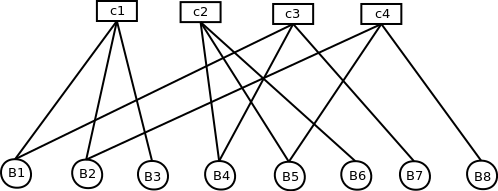
\includegraphics[height=4.5cm,width=10cm]{minSum1}
\caption{ Tanner Graph }
\end{figure}



\subsection{Bit Flipping Decoding} 


 A hard decision is made by the detector for the received bits before passing them to decoder.
Then bits are placed on the bit nodes and passed through the edges of the Tanner graph.
The check node determines that its parity-check equation is satisfied if the modulo-2 sum of the incoming bit values is zero else they pass the flipped value to the corresponding bit.
If the majority of the reception by a bit node are different from its present value then bit node changes (flips) its current value.
This process is repeated until all of the parity-check equations are satisfied, or the decoder gives up.\\
As LDPC matrix is sparse it is unlikely to have same set of checks for a single bit still if several checks applied to single bit are incorrect then it is likely to be flipped. \\
\textbf{Example:} \\
If valid codeword for a Tanner graph is c = [0 0 1 0 1 1] (transmitted code); \\
Received code word is y = [1 0 1 0 1 1] (detected code);\\
The decoding algorithm proceeds as following:

\begin{figure}[h]
  \centering
  \begin{minipage}[b]{0.45\textwidth}
    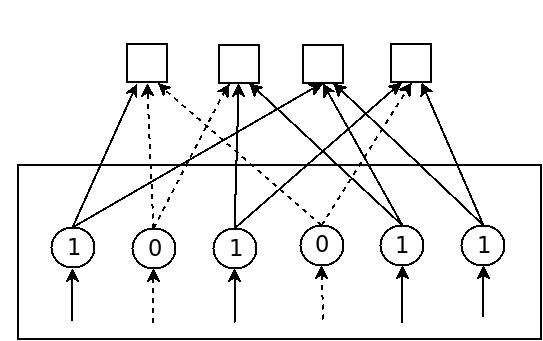
\includegraphics[height=5cm,width=6cm]{initialization}
    \caption{Initialization}
  \end{minipage}
  \hspace{4mm}
  \begin{minipage}[b]{0.45\textwidth}
    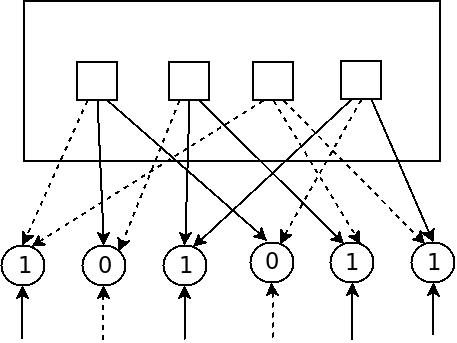
\includegraphics[height=5cm,width=6cm]{PerCheck}
    \caption{Performing Checks}
  \end{minipage}
\end{figure}    

 \begin{figure}[h]
  \centering
  \begin{minipage}[b]{0.45\textwidth}
    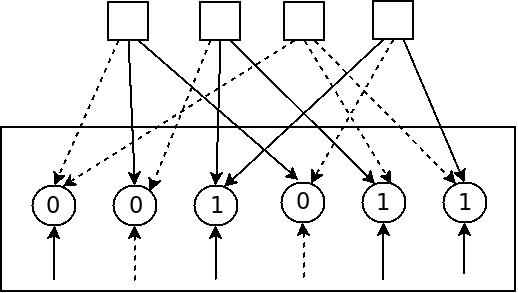
\includegraphics[height=5cm,width=6cm]{BitUpdate}
    \caption{Bit Update}
  \end{minipage}
  \hspace{2mm}
  \begin{minipage}[b]{0.45\textwidth}
    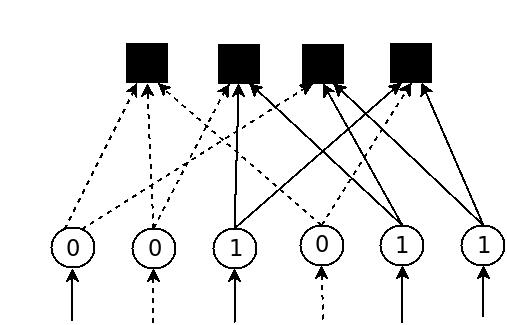
\includegraphics[height=5cm,width=6cm]{Test}
    \caption{Test}
  \end{minipage}
\end{figure}   
 
\subsection{Belief Propagation Decoding (Sum-Product Decoding)} 


It is soft decision algorithm.
Bit-flipping decoding accepts an initial hard decision on
the received bits as input, whereas the sum-product algorithm accepts the probability of each received bit as input.
The input bit probabilities are called the a priori probabilities.
The bit probabilities returned by the decoder are called the a posteriori probabilities.
For sum-product decoding these probabilities are expressed
as log-likelihood ratios (LLR).
\begin{align} L(x)=log\dfrac{p(x=0)}{p(x=1)}=log\dfrac{1-p(x=1)}{p(x=1)} \end{align}
 If p(x = 0) $>$ p(x = 1) then L(x) is positive.
%The greater the difference between p(x = 0) and p(x = 1), i.e. the more
%sure we are that p(x) = 0, the larger the positive value for L(x), and vic. versa.
Log Likelihood Ratios are used to represent the metrics for a binary variable x
by a single value rather than individual probability of being zero and one.
%The sign of L(x) provides the hard decision on x and the magnitude $|L(x)|$ represents
%the reliability of this decision.\\
LLR based representation has benefit when probabilities
need to be multiplied LLR need only be added, reducing the implementation complexity.
The goal is to achieve maximum a posteriori probability of for each bit. 
The extra information about bit i received
from the parity-check j is called extrinsic information for bit i denoted by $E_{j,i}$. The probability ($P_{j,i}^{ext}$ ) that check j is satisfied when ith bit is one is equal to the probability of having odd number of 1s in the check j other than bit i.
\begin{align} P_{j,i}^{ext} = \dfrac{1}{2}-\dfrac{1}{2} \prod_{i'\in B_j, \ i'\neq i }(1-2P_{i'}^{int})  \end{align}
$P_{i'}^{int}$ is a priori probability of ith bit to be 1. Thus,
\[ E_{(j,i)} =  LLR (P_{j,i}^{ext}) = log \left(
\dfrac{1-P_{j,i}^{ext}}{P_{j,i}^{ext}} 
\right)
\]
\[ E_{(j,i)} = log
\left(
\dfrac{\dfrac{1}{2}+\dfrac{1}{2} \prod_{i'\in B_j \ i'\neq i }(1-2P_{i'}^{int}) }{\dfrac{1}{2}-\dfrac{1}{2} \prod_{i'\in B_j \ i'\neq i }(1-2P_{i'}^{int}) } 
\right)
 \]
Using relationship: $tanh \left(  \dfrac{1}{2}log \left( \dfrac{1-p}{p} \right) \right)=1-2p$;
\[ E_{(j,i)} = log
\left(
\dfrac{\dfrac{1}{2}+\dfrac{1}{2} \prod_{i'\in B_j \ i'\neq i }tanh(M_{j,i'}/2) }{\dfrac{1}{2}-\dfrac{1}{2} \prod_{i'\in B_j \ i'\neq i }tanh(M_{j,i'}/2) } 
\right)
 \]
where 
\[ M_{(j,i')} =  LLR (P_{j,i'}^{int}) = log \left(
\dfrac{1-P_{j,i'}^{int}}{P_{j,i'}^{int}} 
\right)
\]
Alternatively, using the relationship
\[ 2tan^{-1}(p)=log \left( \dfrac{1+p}{1-p} \right) \]
%%%%%%%%%%%%%%%%%%%%%%%%%%%%%%%%%%%%%%%%%%%%%
Thus extrinsic information from check j to bit i is:
\begin{align} E_{(j,i)} = 2tan^{-1} \left( \prod_{i'\in B_j ,\ i'\neq i }tanh(M_{j,i'}/2) \right) \end{align}
Total LLR passed to bit i is
\begin{align} L_i = LLR(P_i^{int}) = r_i + \sum_{j\in A_i} E_{j,i} \end{align}
where $r_i$ is input a priori for bit i.
But, message sent again from bit to check avoid the information which checks already have. Thus,
$M_{j,i}$ is not exactly the extrinsic information, it exclude the message generated by the same check node.\\
\begin{align}  M_{j,i} = \sum_{j'\in A_i j'\neq j} E_{j,i} + r_i \end{align}.\\
%\item %Each bit has access to the input a priori LLR, ri, and the LLRs from every
%connected check node. The total LLR of the i-th bit is the sum of these LLRs
After every iteration hard decision is made on the LLR post priori. If code satisfies $Hc^T=0$ then decoding stop else $M_{j,i}$ is found and next iteration is performed.

\subsection{Min Sum Decode}
The min sum decode algorithm is simplification in the sum product algorithm. \\
For BPSK modulation transmitted $0's$ are represented as $-1's$ and transmitted $1's$ are represented as $1's$, calculation soft information:  \\

The probability that bit 1 is received 
\[ f_y(y|f=-1) = \dfrac{1}{\sqrt{2\pi\sigma^{2}}} \exp{\dfrac{-(y+1)^2}{2\sigma^2}}
 \]
 

The probability that bit 0 is received 
\[ f_y(y|f=1) = \dfrac{1}{\sqrt{2\pi\sigma^{2}}} \exp{\dfrac{-(y-1)^2}{2\sigma^2}}
 \]
 
Thus getting LLR as:
 \[  LLR = \log\dfrac{f_y(y|f=-1)}{f_y(y|f=1)} = \dfrac{-2y}{\sigma^2}\]
 
A priori information on the bit node side is expressed in term of LLR as: 
\[  aPriori[I] = -4 * C[I] * R * \dfrac{Eb}{No} \]
where C[I] = $i^{th}$ code block\\
R = code rate\\
$\dfrac{Eb}{No}$ = signal to noise power ratio\\
	
Messages are the information propagating from bit nodes to check nodes.
These are initialized to a priori of their respective bit node.	
 \[ message[I][J] = aPriori[I] \]
 
Extrinsic information of a bit node is calculated min sum of all the message's connected to 
	that particular check node. 
 \[ |E_{(j,i)}| =  Min_{i'\in B_j \ i'\neq i }|M_{j,i'}|   \] 
 \[ sign({E_{(j,i)}}) =  \prod_{i'\in B_j \ i'\neq i }sign(M_{j,i'})   \]
 
A posteriori probabilities are the output bit probabilities.
These are used to modify the code block after every iteration.

\[  aPosteriori[I] = \sum_{j\in A_i} E_{j,i} + aPriori[I] \]
	
Then hard decision is taken on the a posteriori information, that represent the decoded code block.
If decoded code block satisfies $c*H^{T} = 0 $, then decoding stops. Else messages are updated and transmitted back to start the next iteration of decoding.
\[   message_{(j,i)} = aPosteriori[i] - E_{(j,i)}  \]	

\chapter{Results of Software level verification}
\section{Results of Sum Product Algorithm}
\subsection{Random Matrix}

\subsection{Quasi cyclic Matrix}

\section{Results of Min Sum Decode Algorithm}
\subsection{Random Matrix}

\begin{center}
\begin{tabular}{|l|l|r|r|r|r|r|}
\hline
n$\simeq$   & BER(In)$\simeq$    & R=0.75  & R=0.8   & R=0.85  & R=0.9 & R=0.95 \\ \hline
4K  & $1.0x10^{-2}$  &  1.2799$x10^{4}$   & 2.0754$x10^{4}$  & 3.39$x10^{2}$ & 1.259$x10^{3}$ & NA      
\\ 
    & $0.5x10^{-3}$  &  5.53727$x10^{5}$  &  1.72781$x10^{5}$& 6.6700$x10^{4}$ & 1.65511$x10^{5}$ & NA   
\\ 
    & $1.0x10^{-3}$  & -			      & 6.24436$x10^{5}$& 3.45503$x10^{5}$& 1.19008$x10^{5}$  & NA  
\\ \hline
8K  & $1.0x10^{-2}$  & 1.92476$x10^{5}$   & 8.3898$x10^{4}$  & 5.193$x10^{3}$ & 5.947$x10^{3}$         & NA      \\ 
    & $0.5x10^{-3}$ & 3.21027$x10^{5}$    & 4.6092$x10^{4}$& 3.7952$x10^{4}$ & 1.1389$x10^{4}$ & NA  
\\ 
    & $1.0x10^{-3}$ & -				     & -  				 & -         	  & -    & NA             
\\ \hline
12K & $1.0x10^{-2}$ & 2.20022$x10^{5}$   & 1.57371$x10^{5}$  & 1.2894$x10^{4}$ & 1.2626$x10^{4}$     & 1.1      \\ 
    & $0.5x10^{-3}$ & 2.17452$x10^{5}$   & 9.0158$x10^{4}$& 1.56487$x10^{5}$& 5.4866$x10^{4}$ & 1.034$x10^{4}$    \\ 
    & $1.0x10^{-3}$ & -				     & -   & -			  			 & -     & 1.4759$x10^{4}$   \\ \hline
\end{tabular}
\end{center}


\subsection{Quasi cyclic Matrix}

\begin{center}
\begin{tabular}{|l|l|r|r|r|r|r|}
\hline
n$\simeq$   & BER(In)$\simeq$    & R=0.75  & R=0.80  & R=0.85  & R=0.9 & R=0.95 \\ \hline
4K  & $1.0x10^{-2}$  & -    & - &2.677$x10^{3}$           &1.7819$x10^{4}$       &1       \\ 
    & $0.5x10^{-3}$  &-     & - &2.4944$x10^{4}$          &1.65511$x10^{5}$		&1.79$x10^{2}$   \\ 
    & $1.0x10^{-3}$  & -   & -  &5.47550$x10^{5}$         &4.89654$x10^{5}$     &3.328$x10^{3}$ \\ \hline
8K  & $1.0x10^{-2}$   & -   & - &2.3817$x10^{4}$          &1.16847$x10^{5}$        &1   \\ 
    & $0.5x10^{-3}$   & -     & -&6.9491$x10^{4}$          &1.72263$x10^{5}$       &1.001$x10^{3}$  \\ 
    & $1.0x10^{-3}$   & -   & -  &9.16505 $x10^{5}$        &6.28939$x10^{5}$       &9.338$x10^{3}$  \\ \hline
12K & $1.0x10^{-2}$   & -   & -  &9.705$x10^{3}$          &5.37754$x10^{5}$       	&1       \\
    & $0.5x10^{-3}$   & -     & -&5.6400$x10^{4}$          &-     			 		&1.318$x10^{3}$  \\ 
    & $1.0x10^{-3}$   & - & - &- 			             &-    					 &1.6920$x10^{4}$   \\ \hline 
\end{tabular}
\end{center}



\chapter{Partitioning of the Parity Check Matrix}

\section{Introduction}
The literature survey about hardware implementation of the LDPC decoder concludes three different implementation strategies.The serial decoder is the simplest decoder. Hardware cost and complexity is very less. It consists of single check node, single bit node and memory. The bits are first passed one by one from bit side to check side and generated checks are stored in memory, then checks are passed from check side to bit side one at a time to update the bit nodes. The main drawback is this implementation is too slow [5]. The second approach is implementing a fully parallel algorithm. This is a direct implemention of the Tanner graph in hardware [5]. This increases the decoding speed, but hardware cost and implementation complexity becomes too high. Another approach is midway between serial and parallel, called partial parallel implementation. This implementation is more flexible as trade off between speed and cost can be done. In partial parallel implementation bit nodes and check nodes are divided into several partitions. All these partitions works in parallel, but within one partition the information is transferred serially. The larger number of partitions, faster the decoder as it acts more like parallel decoder. The fewer the partition, simpler the decoder as it acts more like serial implementation of the decoder. Thus, we can trade off between speed and cost. Further, a reconfigurable interconnection network has to be designed to change the connection from bit to check side for different iterations in partial parallel decoder. The multistage interconnection network provides cost efficient parallel processing. Non-blocking and rearrangable networks are preferred. In blocking network connection is not always possible, whereas non-blocking network always provides a path between input to output. A rearrangable network can always provide a path, but path has to be rearranged. Lee and Ryu have used Benes network in their partial parallel LDPC decoder [6]. Benes network is a rearrangable network.

\section{Partitioning}
To use the partial parallel approach we propose to iteratively decompose the Tanner graph into sets of bits and sets of checks. In one iteration one set of bits is transferred towards one set of checks. It will be preferred that maximum number of the computational bits required for a particular check set are in same bit set so that computation can be completed for as many check nodes as possible. If a check set requires bits from many bit sets, then the number of iterations required to complete the computation of that set will be equal to the number of bit sets required to perform all the computation. Thus, if many check sets require bits from a large number of bit sets, then number of iterations increases and decoding time will become worse. Thus, an efficient partitioning of bit and check side of the Tanner graph is required. \\
The objective is to partition the bipartite graph corresponding to parity check matrix into two subsets in both bit side and check side such that most of the edges of a set of bit side relates to a particular set of check side. We call these edges as ’Through edges’. The remaining edges of the same set on the bit side that goes to different set in check side are called ’Transverse edges’. The average ratio of total number
of through edges to total number of edges is the performance index for parallelization. \\
Suppose we have bipartite graph G, bits are
B = \{ b\textsubscript{1} ,b\textsubscript{2} ,b\textsubscript{3} ,...,b\textsubscript{n} \} and checks are C=\{ c\textsubscript{1},c\textsubscript{2} ,c\textsubscript{3},...,c\textsubscript{m} \}
and the edge between bit node b i and check node c j is represented as e\textsubscript{i,j}. Now we have to partition G into four subsets B\textsubscript{1} ,B\textsubscript{2} ,C\textsubscript{1} and C\textsubscript{2} such that
\begin{itemize}
\item   Size of set B\textsubscript{1} and set B\textsubscript{2} should be nearly equal as well
as size of C\textsubscript{1} and C\textsubscript{2} should be nearly equal.
\item  There should be a very small number of edges between
B\textsubscript{1}-C\textsubscript{2}and B\textsubscript{2}-C\textsubscript{1}so that the number of cross edges are minimised. 
\end{itemize}


 \begin{figure}[h]
 \begin{center}
    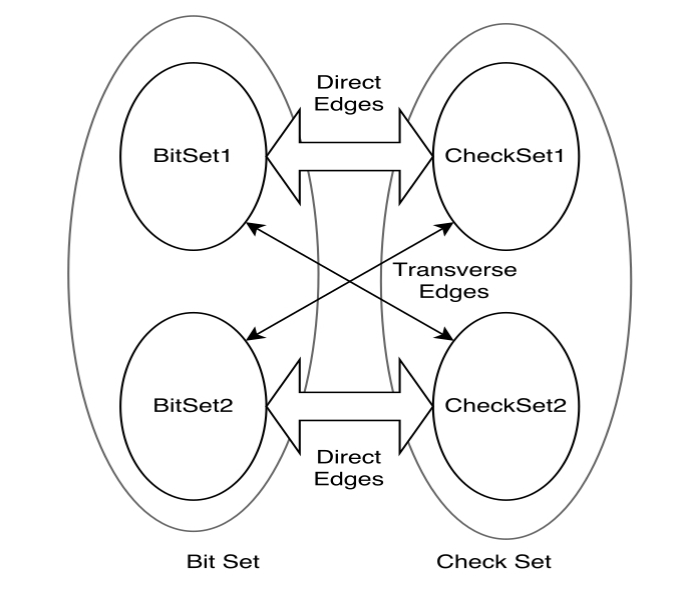
\includegraphics[height=8cm,width=8cm]{partition1.jpg}
    \caption{Partitioning a bipartite graph} 
 \end{center}
\end{figure}


\section{Procedure}
To approach this we initially find a weighted check matrix from the parity check matrix. The weighted check matrix is an incidence matrix for the check node graph. A check node graph is a weighted graph. The weight between checknode\textsubscript{i} and checknode\textsubscript{j} is the number of common bit nodes performing check on both checknode\textsubscript{i} and checknode\textsubscript{j} . After forming the
weighted check graph we partitioned it into two equal parts using METIS [7]. After partitioning the check set into two equal sets with minimum weight cut, we need to partition the bit set. To partition the bit set we take into account the number of checks associated with a bit. If number of checks associated with a bit are more in first check set then it goes to first check set else it goes to second check set. As all matrices are sparse, the number of bits divided in two sets comes out nearly equal. To make them exactly equal we force some bits to go to other set after partitioning. Then the average ratio of parallelized edges to total edges and transverse edges to total edges is calculated as a performance index of parallelization of the
decoder. Figure 4 shows the block diagram for the process of partitioning the bipartite graph corresponding to a low density parity check matrix.


 \begin{figure}[h]
 \begin{center}
    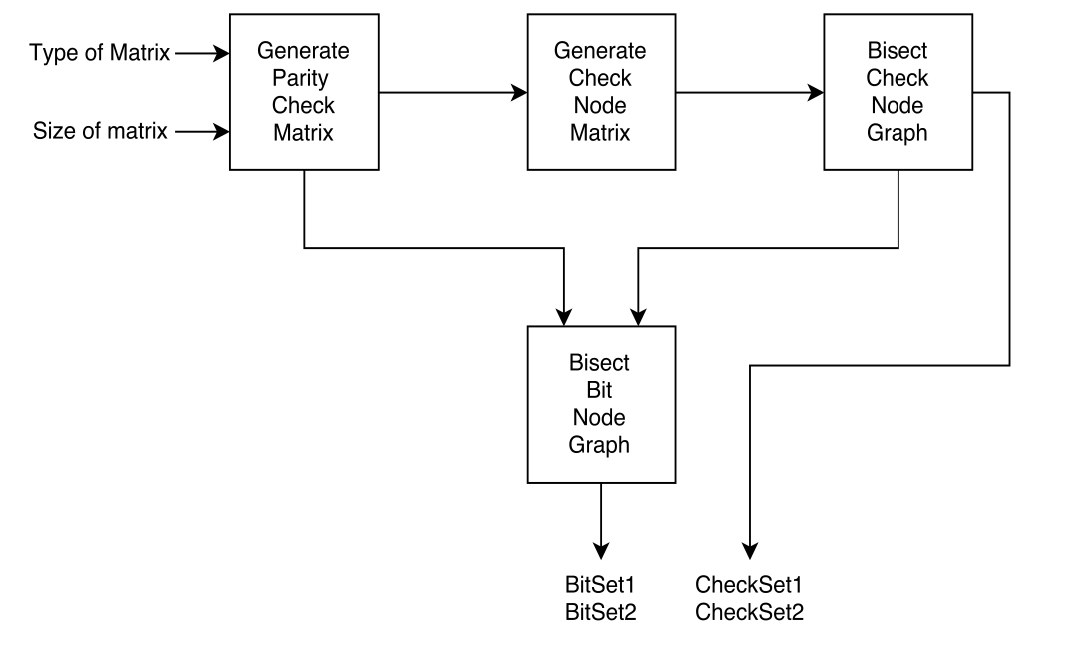
\includegraphics[height=8cm,width=14cm]{partition2.jpg}
    \caption{Block Diagram of process flow} 
 \end{center}
\end{figure}  

\begin{itemize}
\item \textbf{Generation of Parity Check Matrix}
\item \textbf{Generation of Check Node Incident Matrix} \\
The weight between two check nodes is the number of com-
mon bit nodes performing Exor operation on both check nodes.
Taking this into account, we followed following algorithm to
convert a parity check matrix to a check node incidence matrix.

\item \textbf{Bisection of Check Node Graph}

Partitioning of check node graph is done using METIS [7].
METIS is a set of serial programs for partitioning graphs,
partitioning finite element meshes, and producing fill reducing
orderings for sparse matrices. The algorithms implemented in
METIS are based on the multilevel recursive-bisection, mul-
tilevel k-way, and multi-constraint partitioning schemes [7].
First, the incidence matrix is converted into a corresponding
graph format that can be given as input to METIS. At output
we get two partitions of equal size with the minimum weight
cut.

\item \textbf{Bisection of Bit Node Graph}

After bisection of the check set we get two sets C\textsubscript{1} and C\textsubscript{2} .
Now, we have to divide a partition of bit set into B\textsubscript{1} and B\textsubscript{2} . A
bit node corresponds to set B\textsubscript{1} if the number of edges between
that bit node and set C\textsubscript{1} are more than the number of edges
between bit node and set C\textsubscript{2} . As the check set is bisected by
keeping in mind that the more the number of checks relating
to a bit are in same set and the matrix is sparse thus we get
nearly equal bits in set B\textsubscript{1} and set B\textsubscript{2} . As this bisection has
to be further iterated for partitioning, we force the bisection
to be equal. Forcing the bisection to be equal increases the
transverse edges.


\end{itemize}

\section{Results of partitioning applied to matrices}
Simulation for partitioning are performed in MATLAB environment. Figure 5 shows the performance index for Gallager matrix when we vary the order of the parity check matrix from 1,000 to 10,000. The performance index comes 0.78 for Gallager matrix. Similarly, by varying the order of the parity check matrix from 1,000 to 10,000 we get performance index of MacKay Neal matrix as 0.88, depicted in Figure 6. Quasi Cyclic matrix can be formed only for a special set of numbers. In simulation,the order of matrix taken is 155,305,905,11555
and performance index is above 0.88 in all cases, as depicted in Figure 7.

 \begin{figure}[h]
 \begin{center}
    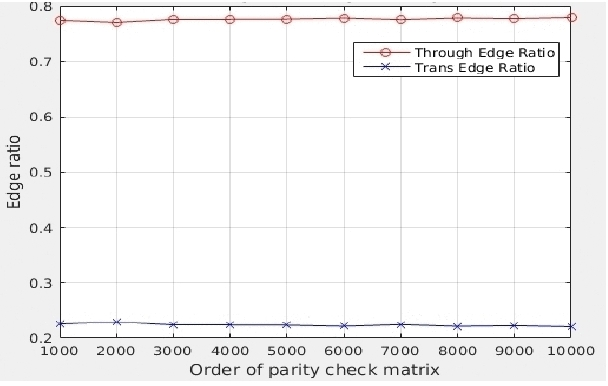
\includegraphics[height=8cm,width=12cm]{gallager_part.jpg}
    \caption{Performance of Gallager matrix} 
 \end{center}
\end{figure}   
 
  \begin{figure}[h]
 \begin{center}
    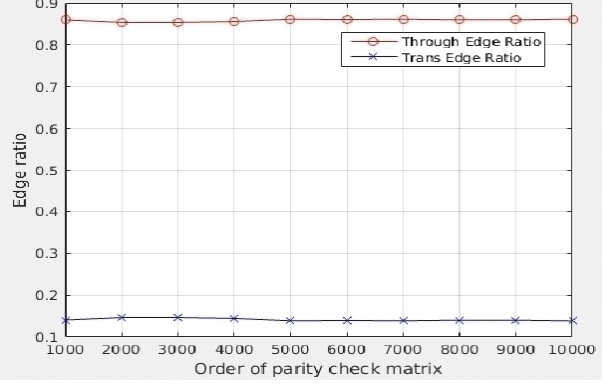
\includegraphics[height=8cm,width=12cm]{makey_part.jpg}
    \caption{Performance of MacKay Neal matrix} 
 \end{center}
\end{figure}


 \begin{figure}[h]
 \begin{center}
    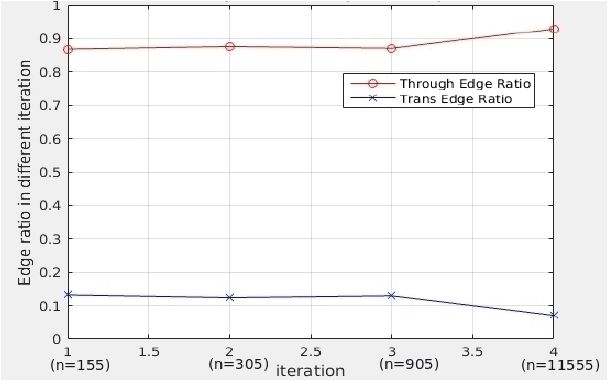
\includegraphics[height=8cm,width=12cm]{qc_part.jpg}
    \caption{Performance of quasi-cyclic matrix} 
 \end{center}
\end{figure}


\chapter{Proposed modification in Min Sum Algorithm using partitioning}



\chapter{Converting Algorithm to hardware using AHIR tool chain}

\chapter{Results and comparisons}

 \begin{thebibliography}{9}
 \bibitem{1} 
 https://wiki.ubuntu.com/LTS.
\bibitem{2} 
 http://www.xilinx.com/kc705 
%\textit{Silicon VLSI Technology: Fundamentals, %Practice and Modeling}. 
%Prentice Hall,2000.
\bibitem{3} 
 Kintex-7 FPGA KC705 Evaluation Kit Getting Started Guide (Vivado Design Suite 2014.3) ( ver6.0, 4932 KB ) [PDF]
 \bibitem{4} 
\verb| http://www.xilinx.com/support/documentation/user_guides/ug344.pdf |
\end{thebibliography}
\addcontentsline{toc}{chapter}{Bibliography}




\end{raggedright}                                                                                                                   
\end{document}
